\documentclass{IEEEtran}
\usepackage[utf8]{inputenc}
\usepackage{graphicx}
\graphicspath{{images/}}
\usepackage{multirow}
\usepackage{array}
\usepackage{hyperref}
\hypersetup{
colorlinks=true,
urlcolor=blue,
citecolor=blue,
pdfpagemode=Fullscreen
}
\title{Bitcoin Closing Price Prediction}
\author
{\IEEEauthorblock{MD. Ahied Mahi Chowdhury, ID: 2018-1-60-028\\ Farhana Alam, ID: 2018-1-60-025\\ Mahtab Hossain, ID: 2018-1-68-005\\ Samia Sultana, ID: 2018-1-60-182}\\
\IEEEauthorblockA{Department of Computer Science Engineering\\
East West University\\
Aftabnagar, Dhaka, Bangladesh\\}
}
\begin{document}
\maketitle

\section{Abstract}
In recent years Bitcoin is a very common crypto currency that has no centralized authority to control it. It is different from the regular stock market. As the price of Bitcoin is very volatile, it is very important to predict the price for investors. We applied Machine Learning algorithms to perform a good prediction over the closing price of Bitcoin. We applied Linear and Polynomial regression and also test the output using cross validation system to find a great output. To perform the project we used python and scikit learn. By observing the output we found that linear regression gave better result than the polynomial regression. By using k-Fold we also train our large data-set to find a good accuracy. As the data-set was very large there were some limitations. We have to face some challenges to plot the graph and we could not able to test higher order polynomial as it needs powerful computers.
\section{Introduction}
Bitcoin is a non-printed form of monetary currency or electronic cash. There is no centralized authority or any third-party financial institutions that have control of the Bitcoin network. All transactions on the Bitcoin network are embedded in blocks. In May 2019 Bitcoin market capitalization value is valued approximately 105 billion of USD which makes it the most valuable crypto currency in the world right now \cite{Uras2020}. The price of Bitcoin is very volatile. Investors are making unthinkable profits sometimes whereas some are going bankrupt. So it is really important to have a good prediction for the investors. 
\subsection{Objective}
This project is going to compare between Multiple Linear Regression and polynomial Regression for different train-test methods and find out their mean absolute error.
\subsection{Motivation}
Bitcoin is different from the traditional stock market. A typical approach in regards to a stock market investment,is Fibonacci retracement.It identifies the opportune moments for traders to buy or sell stock at the optimal price. But Fibonacci retracements are only good metrics for simple identification as the retracement levels are static, and are constant calculated values. For Bitcoin, time series predictions are not a novel idea for brokerage companies, and many brokers have invested heavily to improve performance of forecasting stock prices and foreign exchange rates by way of Machine Learning & Deep Learning \cite{Fahmi2018}. However, It is still not found whether machine learning techniques for the stock market are valid for crypto currencies, this is why working on this topic can be helpful for further analysis in future.
\subsection{Necessity}
Bitcoin is getting popular day by day. The price went up around 250 percent last year. The bitcoin price topped \$60,000 earlier this year before crashing, losing around 40percent of its value in a matter of weeks. It is so volatile that anything can happen anytime. Tesla has bought \$1.5 billion worth of bitcoin and put bitcoin into the corporate radar. payment platforms such as PayPal  and financial technology companies including Jack Dorsey's Square allow users to buy and trade digital assets which helped bitcoin leap. Visa and Mastercard have also indicated  that they're gearing up to offer increased support for bitcoin and cryptocurrencies. Bitcoin is going to sustain its volatility too if a good prediction is not found \cite{Cc}.

\clearpage
\subsection{Existing Works}
\begin{tabular} {|c|c|} \hline
Study & Findings \\ \hline
\multirow{7}{19em}{Regression based Analysis for Bitcoin Price Prediction} & \multirow{7}{19em}{Linear regression gives the best result, mean absolute percentage error for the closing price is 4.095639.} \\ \\ \\ \\ \\ \\ \\ \hline
\multirow{7}{19em} {Predicting Crypto Currency Prices Using Machine Learning and Deep Learning Techniques \cite{Fahmi2018}} & \multirow{7}{19em} {The Recurrent Neural Network model incorporating LSTM cells performed highly accurate than Linear Regression and Linear Regression model with features, having an accuracy of 96.2 percent.} \\ \\ \\ \\ \\ \\ \\ \hline
\multirow{7}{19em}{Forecasting Bitcoin closing price series using linear regression and neural networks models \cite{Uras2020}} & \multirow{7}{19em}{The mean absolute percentage error (MAPE) using Simple Linear regression is 0.007 which is the lowest.} \\ \\ \\ \\ \\ \\ \\ \hline
\multirow{7}{19em}{Bitcoin price prediction using machine learning: An approach to sample dimension engineering \cite{Ee}} & \multirow{7}{19em}{The results show that the statistical methods perform better for low-frequency data with high-dimensional features, while the machine learning models outperform statistical methods for high-frequency data.} \\ \\ \\ \\ \\ \\ \\ \hline
\multirow{10}{19em}{Automated Bitcoin Trading Via Machine Learning Algorithms \cite{Madan}} & \multirow{7}{19em}{Predicting future price with an accuracy of 50 percent in every 10 min interval.} \\ \\ \\ \\ \\  \hline
\multirow{7}{19em}{Predicting short-term Bitcoin price fluctuations from buy and sell order \cite{Dd}} & \multirow{7}{19em}{XGT and regularized regression ENET performed better than others.} \\ \\ \\ \\ \\ \\ \\ \hline
\multirow{7}{19em}{Comparative Performance of Machine Learning Algorithms for Cryptocurrency Forecasting \cite{Hitam2018}} & \multirow{7}{19em}{Highest accuracy of SVM.} \\ \\ \\ \\ \\  \hline
\multirow{7}{19em}{Using the Bitcoin Transaction Graph to Predict the Price of Bitcoin \cite{Greaves2015}} & \multirow{7}{19em}{Regular ANN predicted price direction with an accuracy of 55 percent.} \\ \\ \\ \\ \\ \\ \\ \hline

\end{tabular}
\clearpage

\section{Methodology}
\\ To set about the study into Bitcoin price prediction, we have applied Regression, an effective Machine Learning algorithm that brings a good prediction model. Regression analysis is a technique that can be used for prediction and it explores the bonding between a dependent and independent variable. By using the bonding between the variables, the regression model finds out the best fit line which can be utilized for making predictions. Regression can be classified in many types such as ‘Linear Regression’, ‘Logistic Regression’, ‘Polynomial Regression’, Multi Linear Regression”, and so on \cite{Pant2019}. Among them we have chosen Multi Linear Regression and Polynomial Regression to perform the closing price prediction of Bitcoin.

 Linear regression is one of the most common Machine Learning algorithms basically used for prediction. Linear regression works with continuous data. The general equation of linear regression is-

Simple Linear Regression equation:       y = b0+b1x+E

Multiple Linear Regression equation:     y= b0+b1x1+ b2x2+ b3x3+....+ bnxn +E \cite{Aa}.

Here the dependent variable “y” is the actual output. b0 is the y intercept and bn is called the parameters and also known as weights. Its transpose executes matrix multiplication on an independent variable x. To reduce the mean squared error the value of weights change simultaneously by using the Normal Equation or the Gradient Descent which is profitable for large datasets\cite{Vaddi2020}.

\begin{right}
\centering
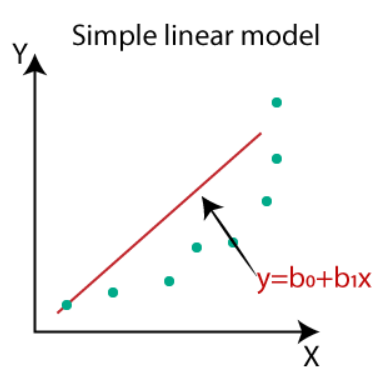
\includegraphics[scale=1]{linear.PNG}
\\\caption{Fig 1: Linear Regression} \\

\end{right}

Polynomial Regression is one kind of a regression algorithm that makes the relationship between a dependent and an independent variable of nth order. The general equation of Polynomial Regression is-

y= b0+b1x1+ b2x12+ b2x13+...... bnx1n+E

Here, y is the dependent variable and b is the weight which is multiplied with the independent variable x1 \cite{Aa}.“n” is the number of order in this equation. Polynomial regression can be used when the value and explanatory variable has a curvilinear relationship\cite{Vaddi2020}.It can fit a large range of functions but if there are any outliers that can be very sensitive for polynomial regression\cite{Pant2019}[Figure\ref{fig_PolynomialRegression}].

\begin{left}
\centering
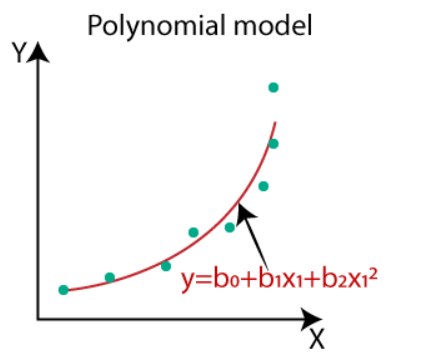
\includegraphics[scale=1]{polynomial.PNG}
\\\caption{Fig 2: Polynomial Regression}\\
\label{fig_PolynomialRegression}
\end{left}

In our project, we split the data set into the test and train set for both the linear and polynomial regression. For the polynomial regression the highest order was 3. After training we got the predicted values and could compare with the actual values. To determine the errors of our project, we have used scikit learn which is very easy to write and understand. It is also very fast to compute. By using the built-in functions we had determined the max error, mean squared error and mean absolute error. 

We also applied the k-Fold cross validation procedure to Linear and polynomial regression for getting better results. Cross validation procedure has a parameter known as k that sets the number of groups that a data set can be splitted. For example if the value of k=10 means it will split the dataset into 10 folds. It shuffles the dataset and splits it into k numbers of groups. From the k groups it sets a group for test set and rest of them for training data set	. It works like a loop over the dataset and covers all the values as it is not a biased procedure. Each group can be set as a test set for once. Generally when k is 5,8 or 10, it gives the best results \cite{Bb}. It gives us the best mean absolute error.

\section{Implementation}
\subsection{Data Collection}
we have collected the dataset from Kaggle from the following link: \url{https://www.kaggle.com/mczielinski/bitcoin-historical-data?fbclid=IwAR2thOvn1-Is3I6-9UgYgvrqAlbu_vadln6-LPcuOJMaNMV290arcPAsUAg}
\subsection{Data Processing}
We have ignored any incomplete data. To get rid of the incomplete row we had to run the following[Figure\ref{fig_incompleteData}].

\begin{figure}
\centering
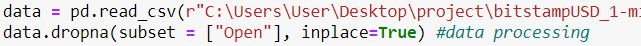
\includegraphics[width = .5\textwidth,length = .7\textlength]{Capture.JPG}
\caption{code for removing incomplete data}
\label{fig_incompleteData}
\end{figure}
\subsection{Model Development}

We have implemented our project in Jupyter notebook using Python.
\subsection{Result}
Mean absolute error of each algorithm on different train test method: \\
\\

\begin{tabular} { | m{15em} | m{5em}| m{5em} | m{5em} | m{3em}| m{3em} | m{3em} | } 
\hline
Algorithm & Train Test split ration 80:20 & Train Test split ration 88:12 & Train Test split ration 90:10 & K-fold K=5 & K-fold K=8 & K-fold K=10 \\
\hline
Multiple Linear Regression & 1.6 & 1.6 & 1.6 & 1.61 & 1.59 & 1.59 \\
\hline
Polynomial Regression(Degree = 2) & 37.0 & 213.9 & 25.7 & 1468.68 & 947.71 & 958.43 \\
\hline
Polynomial Regression(Degree = 3) & 295.1 & 56.3 & 23.3 & 1987.32 & 1954.33 & 1972.38 \\
\hline

\end{tabular}
\\
\\\\From the output we got that our project worked better in Multiple Linear Regression.At first when we split the data set into 80:20 for train and test we got the mean absolute error for the MLR is 1.6 where 2 degree polynomial regression gave 37 and 3 degree polynomial regression gave 295.1 which very higher than the MLR. When we increase the split ratio for train and test, polynomial regression performed better than previous result but it couldn't perform better than the Multiple Linear Regression. 
When we used k-Fold cross validation method, we tested for 5 fold,8 fold and 10 fold. For these three cases, 8 fold performs the best for Multiple Linear Regression.\\
\section{Conclusion}
In this paper we have tried a few Machine Learning approaches to predict the closing price of crypto currencies like Bitcoin. We compared the results with Linear and Polynomial regression and also applied cross validation and compared them. By this research we provide a comparative result and findings that may help to predict the price of crypto currency markets. From our result among the linear and polynomial regression, we get the best result for Linear regression. The main difference between Linear regression and polynomial regression is that the linear regression equation’s highest power is 1 where the polynomial equation’s power is greater than 1. In terms of analysis the order of polynomial models should be kept the lowest. If 1st order doesn't give the best result then higher order has to be applied. Because higher order’s arbitrary fitting may become an abuse in the regression method \cite{Shalabh}. Though polynomial regression can fit larger data but outliers can seriously affect the output in polynomial regression \cite{Pant2019}.From our cross validation process we found that 8-fold gives the best result where all the datasets are splitted into 8 groups. Among the groups each fold works as a train set for once and lastly gives the best accuracy. 
\clearpage
\subsection{Challenges and Limitations}
We worked with a large dataset. We had 48 lacs of data with incomplete data. After the data processing we got around 36 lacs of valid data. For this large amount of data we were unable to generate graphs of our linear and polynomial regression. Higher order polynomial equations need more powerful computers than we have. In our computer we were able to set the order limit upto 3.
\subsection{Future Directions}
We didn’t cover all the machine learning algorithms in our research. In the future we can apply more ML methods like MLP, RNN, Statistical method to test if we get better accuracy rate. Addition of multiple features may increase the performance of Bitcoin closing price prediction.

\bibliographystyle{plain}
\bibliography{ref1}

\end{document}
